\documentclass[onecolumn, draftclsnofoot,10pt, compsoc]{IEEEtran}
\usepackage{graphicx}
\usepackage{url}
\usepackage{float}
\usepackage{setspace}
\usepackage{caption}

\usepackage{geometry}
\geometry{textheight=9.5in, textwidth=7in}

% 1. Fill in these details
\def \CapstoneTeamName{		Nexusphere}
\def \CapstoneTeamNumber{		48}
\def \GroupMemberOne{			Meghan Mowery}
\def \GroupMemberTwo{			Louis Duvoisin}
\def \GroupMemberThree{			Sarahi Pelayo}
\def \CapstoneProjectName{		A-Frame Live Stream Portal}
\def \CapstoneSponsorCompany{	Oregon State University}
\def \CapstoneSponsorPerson{		Behnam Saeedi}

% 2. Uncomment the appropriate line below so that the document type works
\def \DocType{	%Problem Statement
				%Requirements Document
				%Technology Review
				%Design Document
				Progress Report
				}
			
\newcommand{\NameSigPair}[1]{\par
\makebox[2.75in][r]{#1} \hfil 	\makebox[3.25in]{\makebox[2.25in]{\hrulefill} \hfill		\makebox[.75in]{\hrulefill}}
\par\vspace{-12pt} \textit{\tiny\noindent
\makebox[2.75in]{} \hfil		\makebox[3.25in]{\makebox[2.25in][r]{Signature} \hfill	\makebox[.75in][r]{Date}}}}
% 3. If the document is not to be signed, uncomment the RENEWcommand below
%\renewcommand{\NameSigPair}[1]{#1}

%%%%%%%%%%%%%%%%%%%%%%%%%%%%%%%%%%%%%%%
\begin{document}
\begin{titlepage}
    \pagenumbering{gobble}
    \begin{singlespace}
    	\includegraphics[height=4cm]{coe_v_spot1}
        \hfill 
        % 4. If you have a logo, use this includegraphics command to put it on the coversheet.
        %\includegraphics[height=4cm]{CompanyLogo}   
        \par\vspace{.2in}
        \centering
        \scshape{
            \huge CS Capstone \DocType \par
            {\large\today}\par
            \vspace{.5in}
            \textbf{\Huge\CapstoneProjectName}\par
            \vfill
            {\large Prepared for}\par
            \Huge \CapstoneSponsorCompany\par
            \vspace{5pt}
            {\Large\NameSigPair{\CapstoneSponsorPerson}\par}
            {\large Prepared by }\par
            Group\CapstoneTeamNumber\par
            % 5. comment out the line below this one if you do not wish to name your team
            \CapstoneTeamName\par 
            \vspace{5pt}
            {\Large
                \NameSigPair{\GroupMemberOne}\par
                \NameSigPair{\GroupMemberTwo}\par
                \NameSigPair{\GroupMemberThree}\par
            }
            \vspace{20pt}
        }
        \begin{abstract}
        % 6. Fill in your abstract    
        	A-Frame Live Stream Portal is a project that will be used to bring families closer together, even when adversity keeps them apart.
        	This report is a summary of all of the team's achievements this term, including the project, the progress the team has made toward completing the project, and any problems the team has faced. 
        	This report is separated into four main sections, the introduction of our project and the project goals, the week-by-week progress reports in the form of a table, a description of our current prototype, and how much of the project is completed.
        \end{abstract}   	 
    \end{singlespace}
\end{titlepage}
\newpage
\pagenumbering{arabic}
\tableofcontents
% 7. uncomment this (if applicable). Consider adding a page break.
\listoffigures
%\listoftables
\clearpage

% 8. now you write!
\section{Introduction}
    \subsection{Project purpose}
    The supreme court decided in a 5-to-4 vote to support President Trump’s travel ban and restrictions on people from Iran, Libya, North Korea, Somalia, Syria, Venezuela and Yemen traveling into the United States of America \cite{IEEEhowto:TravelBan}. 
    It is estimated that one million Iranian American citizens live in the United States. 
    The number is so high because Iran produces more visas than the other countries. 
    The issue now comes when relatives in Iran want to visit their families in America.
    Jamal Abdi, vice president of policy at the national Iranian American Council, points out that, to travel, Iranians must go through an unpredictable process to obtain a waiver \cite{IEEEhowto:TravelBan}. 
    The uncertainty of obtaining the waiver makes it almost impossible for Iranian people to travel to the United States for the time being. 
    Behman Seedi's family would like to attend his wedding, however their travel plans are disrupted by the improbable chance of getting past the travel ban. 
    To accommodate for them not being there physically, our sponsor wishes to create a system where the family can still view the wedding.
    The main problem that will be solved by giving an immersive, and complete experience while also considering distance, and efficiency.
    Since the sponsor's family lives in another country, we will need to research possible issues with bandwidth, delay during live streaming, and time-zone differences.
    We also need the solution to be efficient or else the family might miss an important part of the wedding due to a delay in the streaming.
    Another problem that will have to be solved is the possibility of a delay between audio and visual output. 
    This delay would make the experience not as enjoyable for a viewer as it could be challenging to understand what is happening during the ceremony if the audio is not in sync with the video.
    To solve this problem, the sponsor suggests that we create an interactive web portal. 
    Wedding preparation is stressful, so we will need to make the project simple enough so the sponsor is not stressed about the project. 
\newline 
    \subsection{Project goals}
     Our desire is to create a system that is more interactive than traditional forms of wedding videography and photography.
    Normal wedding pictures and video need to be edited which can take days and relatives will have missed the events taking place.
    To include our sponsor's absent family, the wedding will instead be streamed live. 
    The solution for this problem is combining a web portal with various cameras that the relatives can select which will allow them to view the proceedings.
    We will create an attractive website with an intuitive interface which will allow those tuning in to explore the venue using a complete map by clicking on the device icons. 
    The map must also have an edit mode which gives it the capability of being updated, letting the camera's locations be moved to different parts of the venue, as well as giving it the option to add or remove cameras at will.
    The web portal will need to be simple and easy to understand so usability does not become an issue for the family viewing the wedding.
    The web portal will be developed using Linux as the operating system, Apaches as the web server, MySQL as the relational database, PHP as the scripting language, and Javascript in conjunction with a Mozilla A-Frame as a framework for handling the 360 video stream. 
\newline
\newline
    Another part of the solution will be the cameras themselves; we want to make them sturdy to reduce the risk of them falling over and breaking. 
    The cameras will broadcast to a website that will be streaming everything in real time at a minimum of three locations. 
    One of the cameras will also have 360 degree video streaming capability that will provide the relatives an even more immersive experience than looking at wedding photos days later. 
    The streaming devices will be positioned around the venue and will have their own internet connection so that they can stream their video feed.
    Therefore these cameras will also need their own WiFi modules and work independently.
    The cameras will have at least 1080p at 30fps stream quality, they will also need to be portable, and easy to set up.
    The ideal choice would then be to use batteries to allow for ease of use and, being portable, we would not be able to have any type of wires connected to them.
    The batteries will either need to be easily swappable, or be large enough to power the cameras for the entire duration of the wedding ceremony.
    Our hope is that the family will have an enjoyable experience that they would not be able to have in other circumstances.
    \pagebreak 
\subsection{Retrospective}
        \begin{tabular}{p{0.3\linewidth}  p{0.3\linewidth}  p{0.3\linewidth}}
         \centering Positives & \centering Deltas & \centering Actions \\
         \end{tabular}  
         
         \begin{tabular}{p{0.3\linewidth} | p{0.3\linewidth} | p{0.3\linewidth}}
         As a group we have met multiple times to understand the problem and discuss our processes for moving forward. We have organized a weekly time to meet with our TA and our sponsor.&
         The problem statement is due next week and needs to be worked on.&
         At this point we didn't have any problems and the only actions that were taken was setting up a meeting time to work on the problem statement.\\
         \hline 
         We met in the library as a group to complete our problem statement. We also met with our client and TA to talk about how things were going and the requirements document. We did some basic research on what hardware we would use for the cameras as well as the streaming.&
         The requirements document is due in two weeks and needs to be worked on.&
         More research on hardware needed to be done and we made a meeting time for our group to start working on the requirements document.\\
         \hline 
         We have completed most of the requirements document and have also begun discussing the tech review. We did research on what technologies we would use preparing for the tech review.&
         The requirements document is due next week and needs to be worked on. The tech review is also due in the near future and needs to be worked on individually. &
         We set up another meeting for finishing up the requirements document and split up what we would write about for the tech review.\\
         \hline
         We have been meeting with our client regularly so far. When we met with him Ben gave us some pointers on what he would like to see changed on the system requirements document. As a team we then discussed it and and made the necessary edits. We completed our requirements document, and delegated what we needed to research for the tech review. After our client meeting we got a Raspberry Pi from Dr. McGrath to start testing streaming options with.&
         We need to complete the paper prototype for the web portal so we can discuss with our client the specifications of the web-page before we create a lightweight prototype. &
         We are planning on meeting to complete the paper prototype within the next week.\\ 
         \hline 
         \end{tabular}
         \newpage
         \begin{tabular}{p{0.3\linewidth} | p{0.3\linewidth} | p{0.3\linewidth}}
         We finished the paper prototype and showed it to our client. During that meeting we got important feedback to use for the lightweight prototype. We also got a Raspberry Pi and camera module to start testing streaming options.&
         We need to make a lightweight prototype of our website. We also need to start testing out different streaming options.&
         We need to look in to software to use to make the prototype as well as actually do the work making it. We also need to do research to find out what options are available for streaming on a Raspberry Pi, and then actually implement those.\\
         \hline
         We created the lightweight prototype based on the paper prototype. We had a client meeting with only Ben where the lightweight prototype was present. We walked through the prototype and emailed to Ben so that he can share it with Jenna. We began working with the raspberry pi by putting an OS on it trying to get it to first take a picture then next take video.&
         We are experiencing some problems with streaming quality on the raspberry pi because the frames per second were far too low. We managed to get 2fps but we need about 30fps. &
         To solve the frame rate streaming problem, we will need to test the raspberry pi further before we decide to purchase another system.\\
         \hline
         Due to the holiday we did not meet with our client nor our TA this week. We instead meet as a group to discuss work we want to do over winter break. We set up our environment where we will begin to code because we agreed to start the website over winter break. We then met again to work on the progress report and video. &
         We are still working with Raspberry Pi to increase the rate of frames per second.&
         While we have not solved our issue with streaming, we found a tutorial which uses a different method and promises a higher frame rate.\\
        \end{tabular}    
        \pagebreak
    
\section{Prototype}
        We made a lightweight prototype of what our website will look like. The version we presented to our client is interactive and clicking on the buttons bring the user to that page. We have received visual feedback on this prototype as well, but have not yet gone back and edited the prototype to match.
        \begin{figure}[H]
            \centering
            \captionsetup{justification=centering,margin=2cm}
            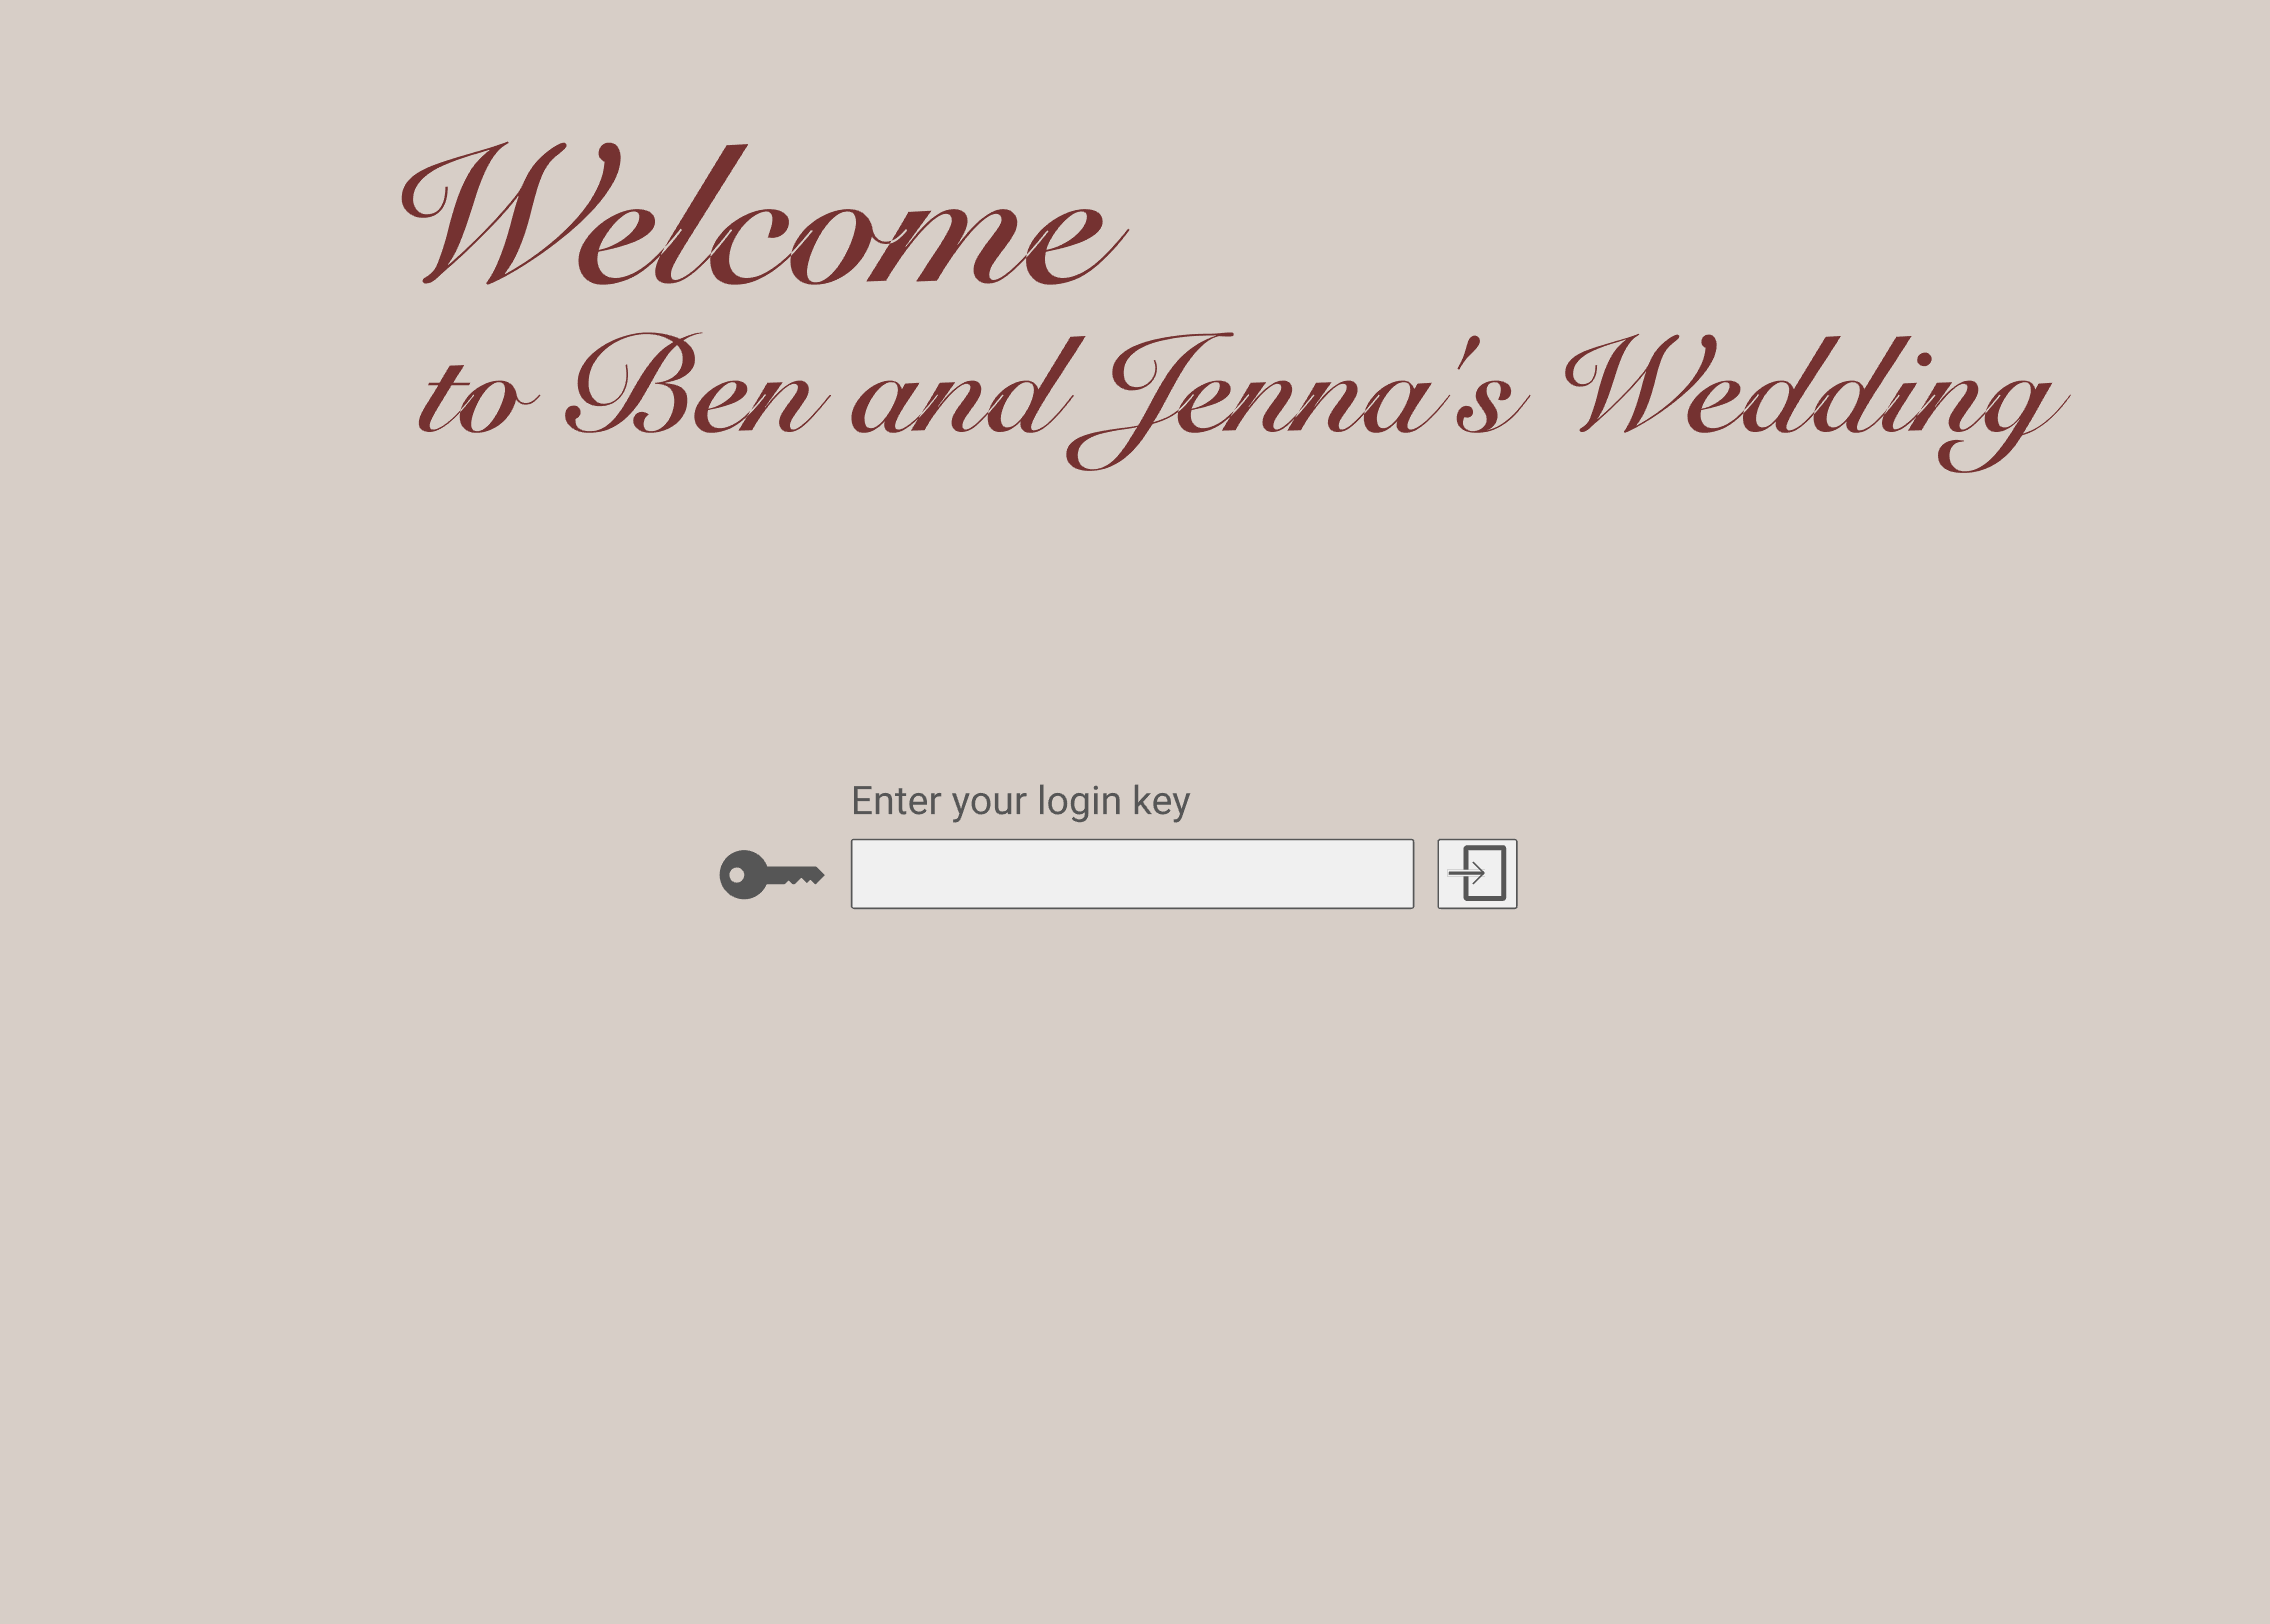
\includegraphics[scale=0.2]{Images/desktop-login.png}
            \centering\caption{Login Page}
            \label{fig:Login}
        \end{figure}
        \begin{figure}[H]
            \centering
            \captionsetup{justification=centering,margin=2cm}
            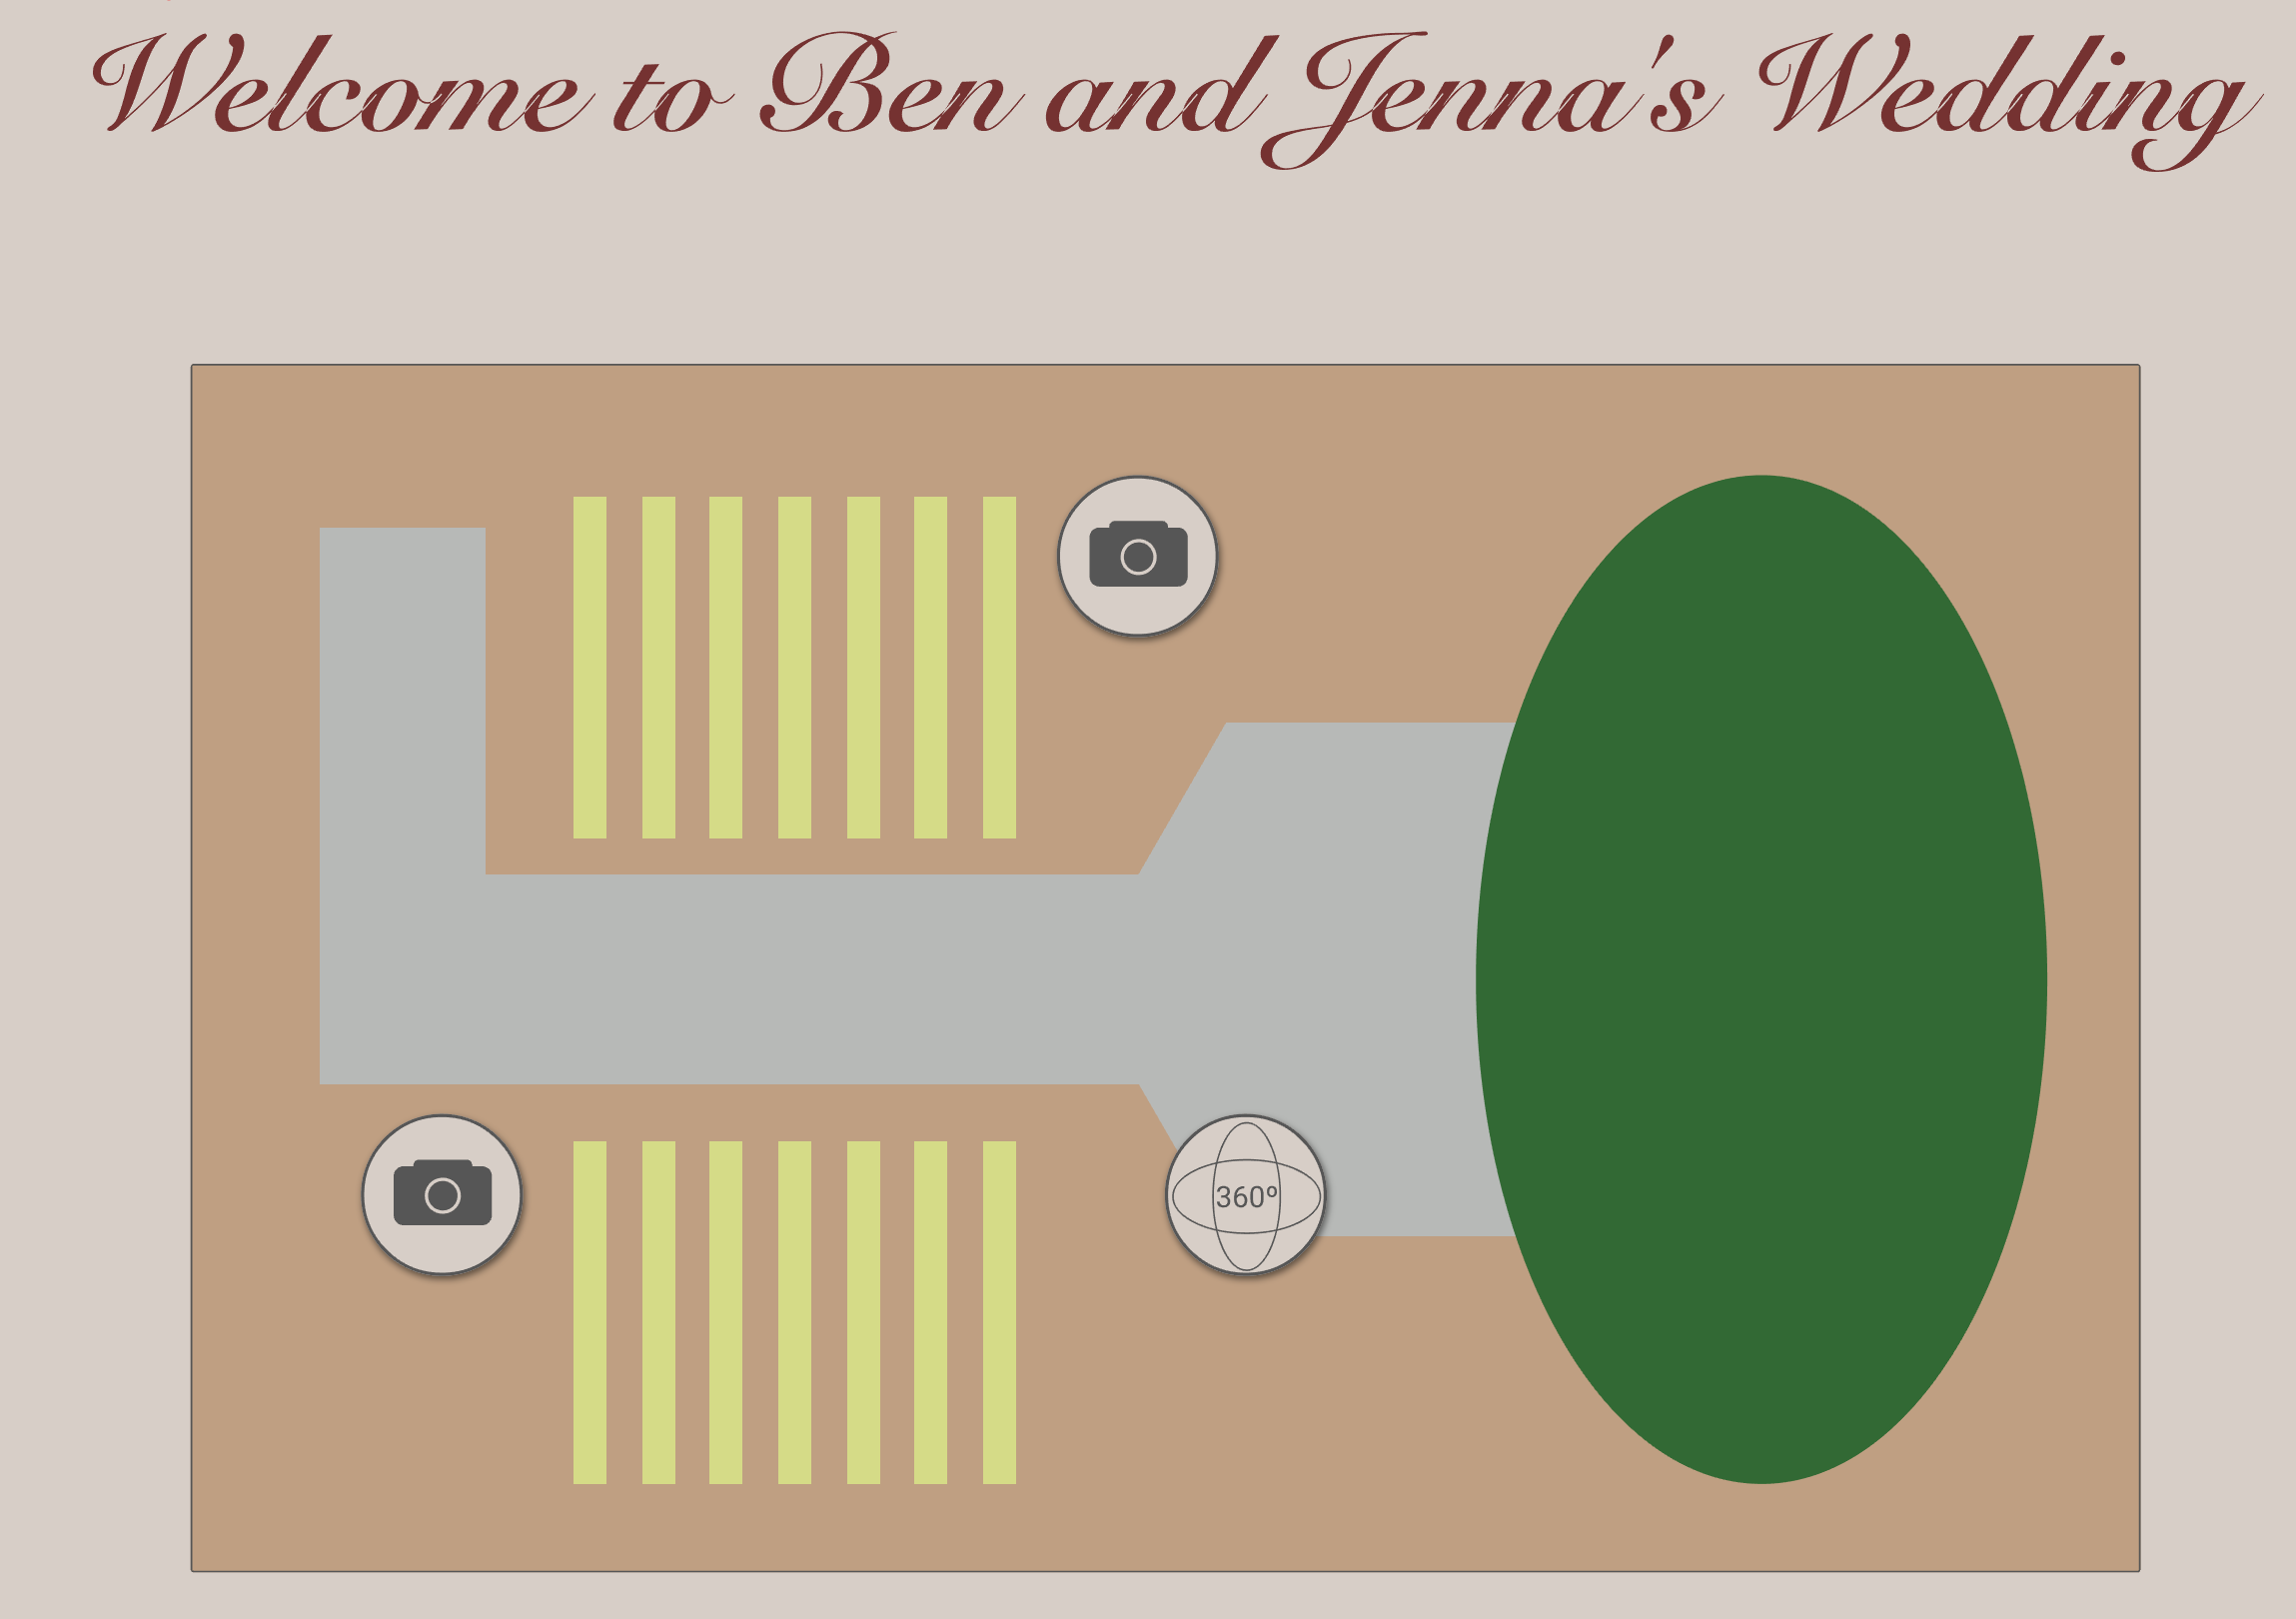
\includegraphics[scale=0.2]{Images/desktop-main.png}
            \centering\caption{User View}
            \label{fig:User}
        \end{figure}
        \begin{figure}[H]
            \centering
            \captionsetup{justification=centering,margin=2cm}
            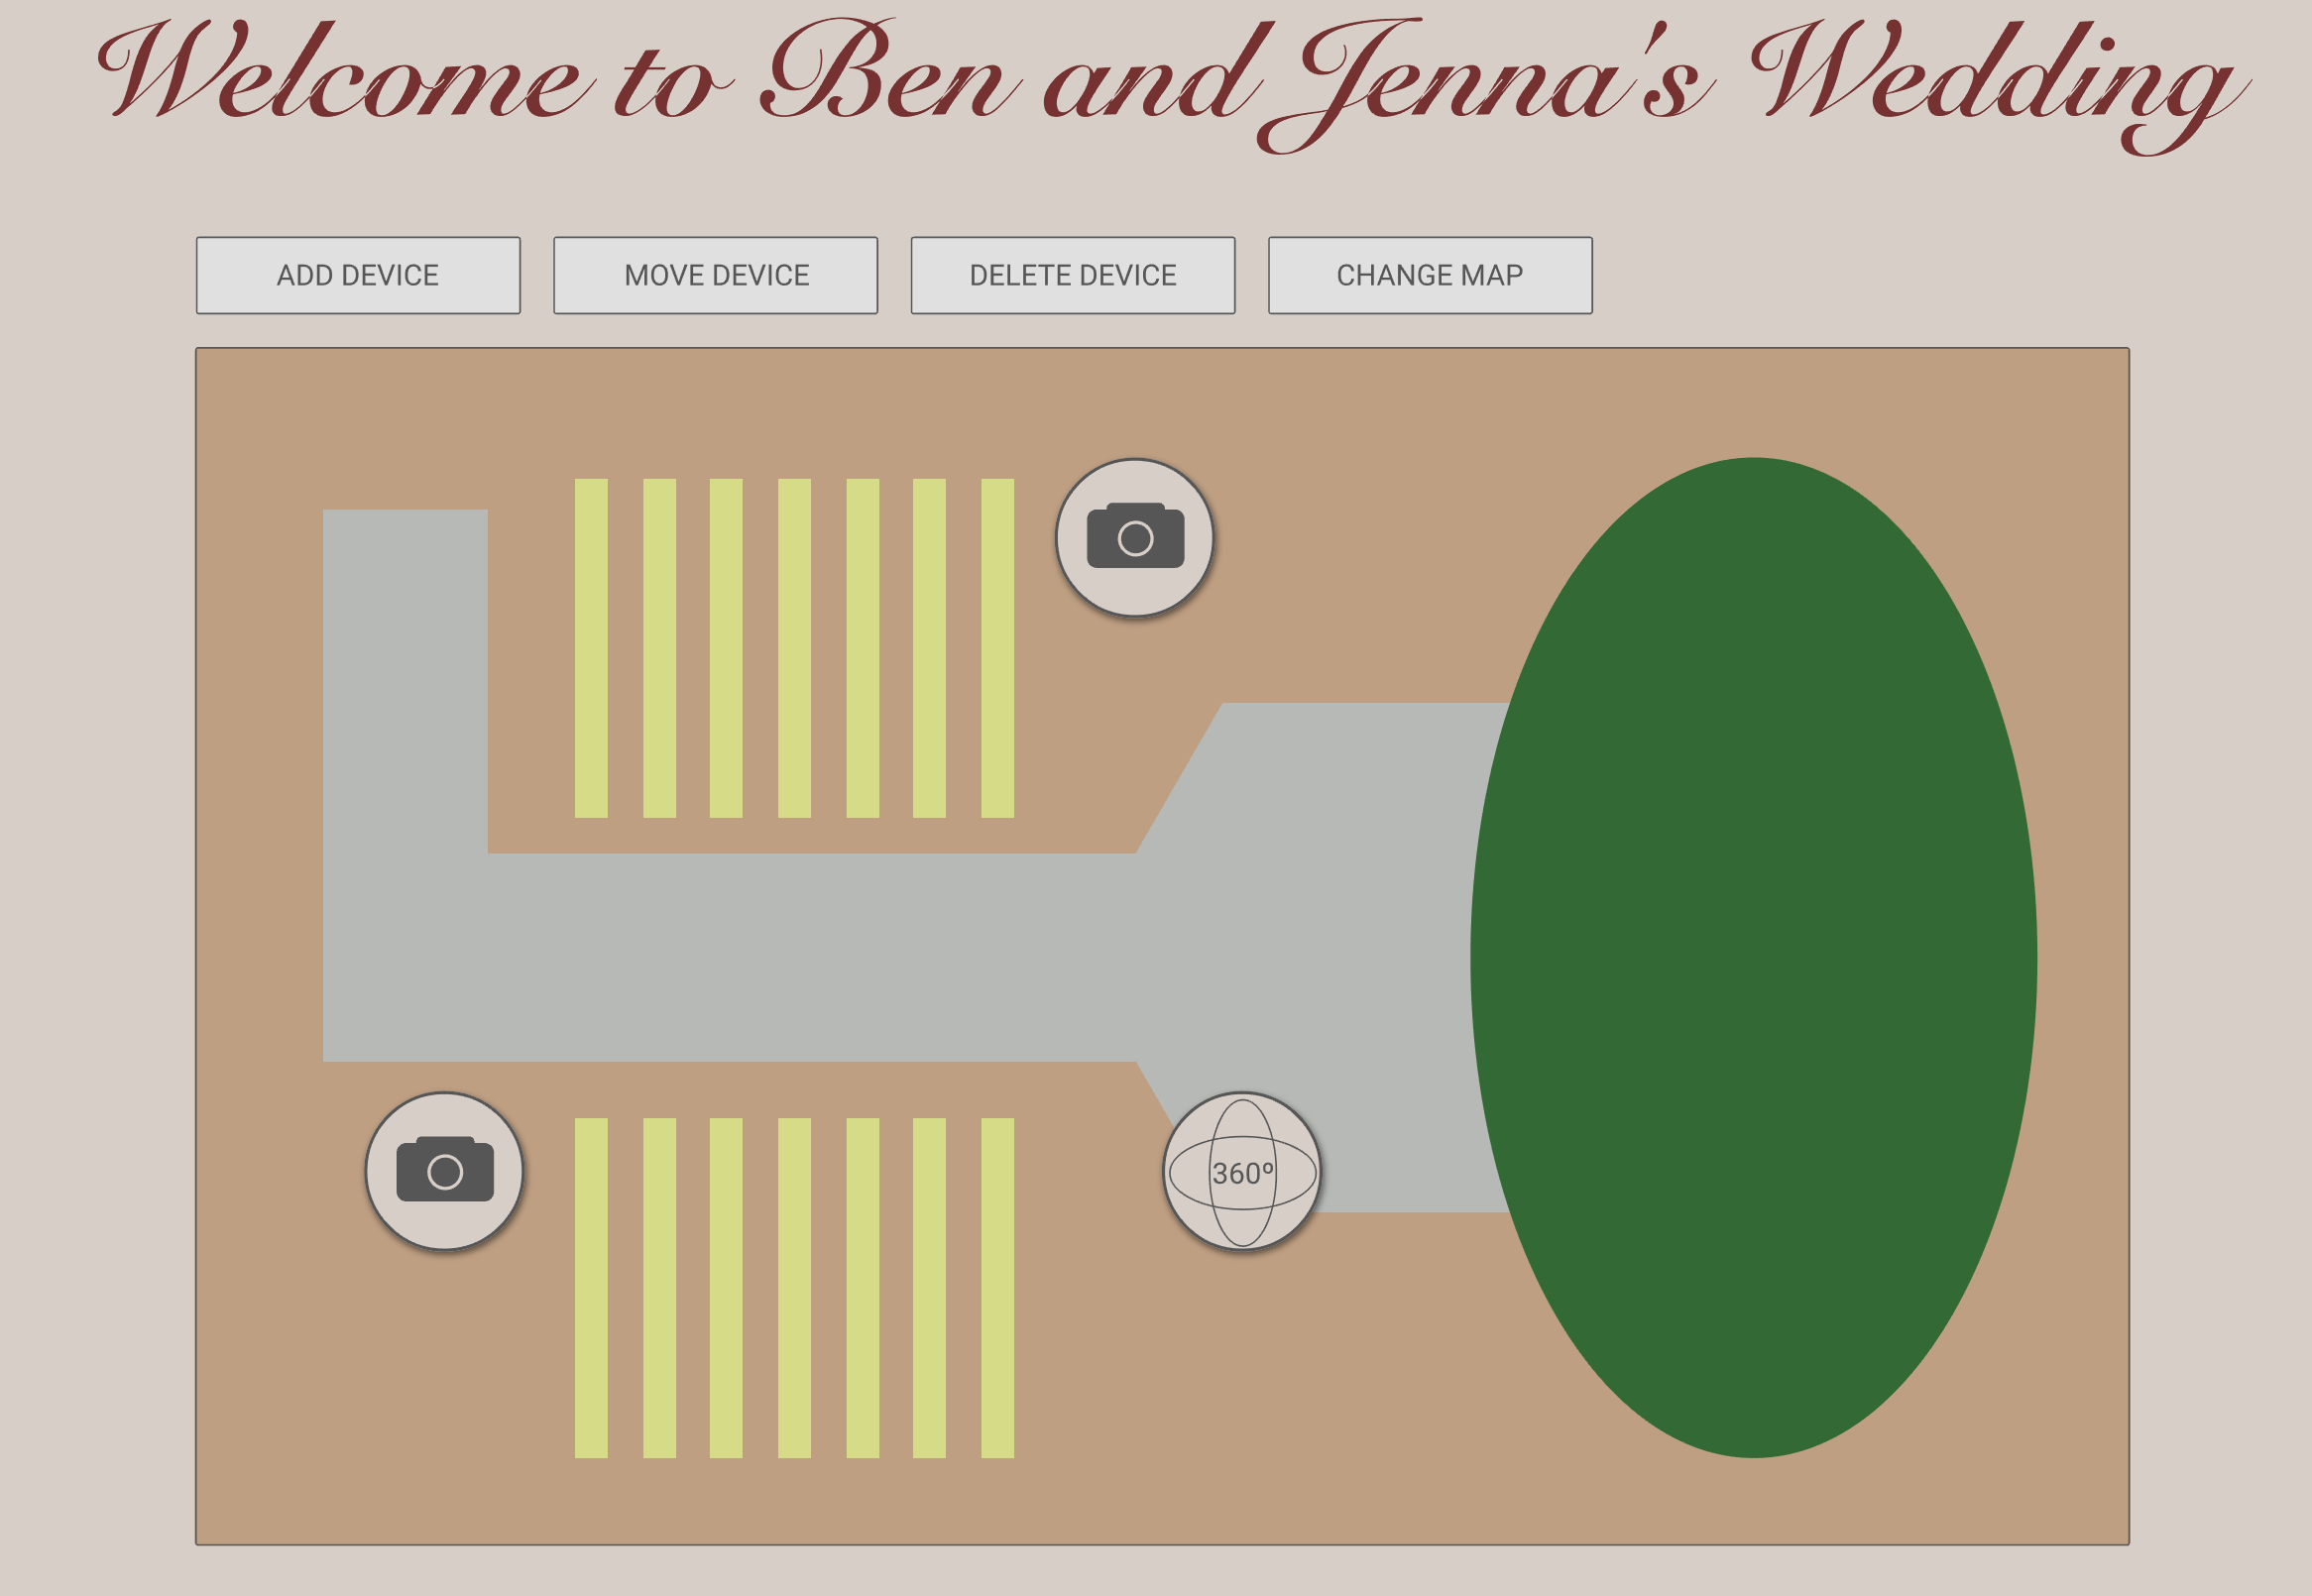
\includegraphics[scale=0.2]{Images/desktop-admin.png}
            \centering\caption{Admin View}
            \label{fig:Admin}
        \end{figure}
        \begin{figure}[H]
            \centering
            \captionsetup{justification=centering,margin=2cm}
            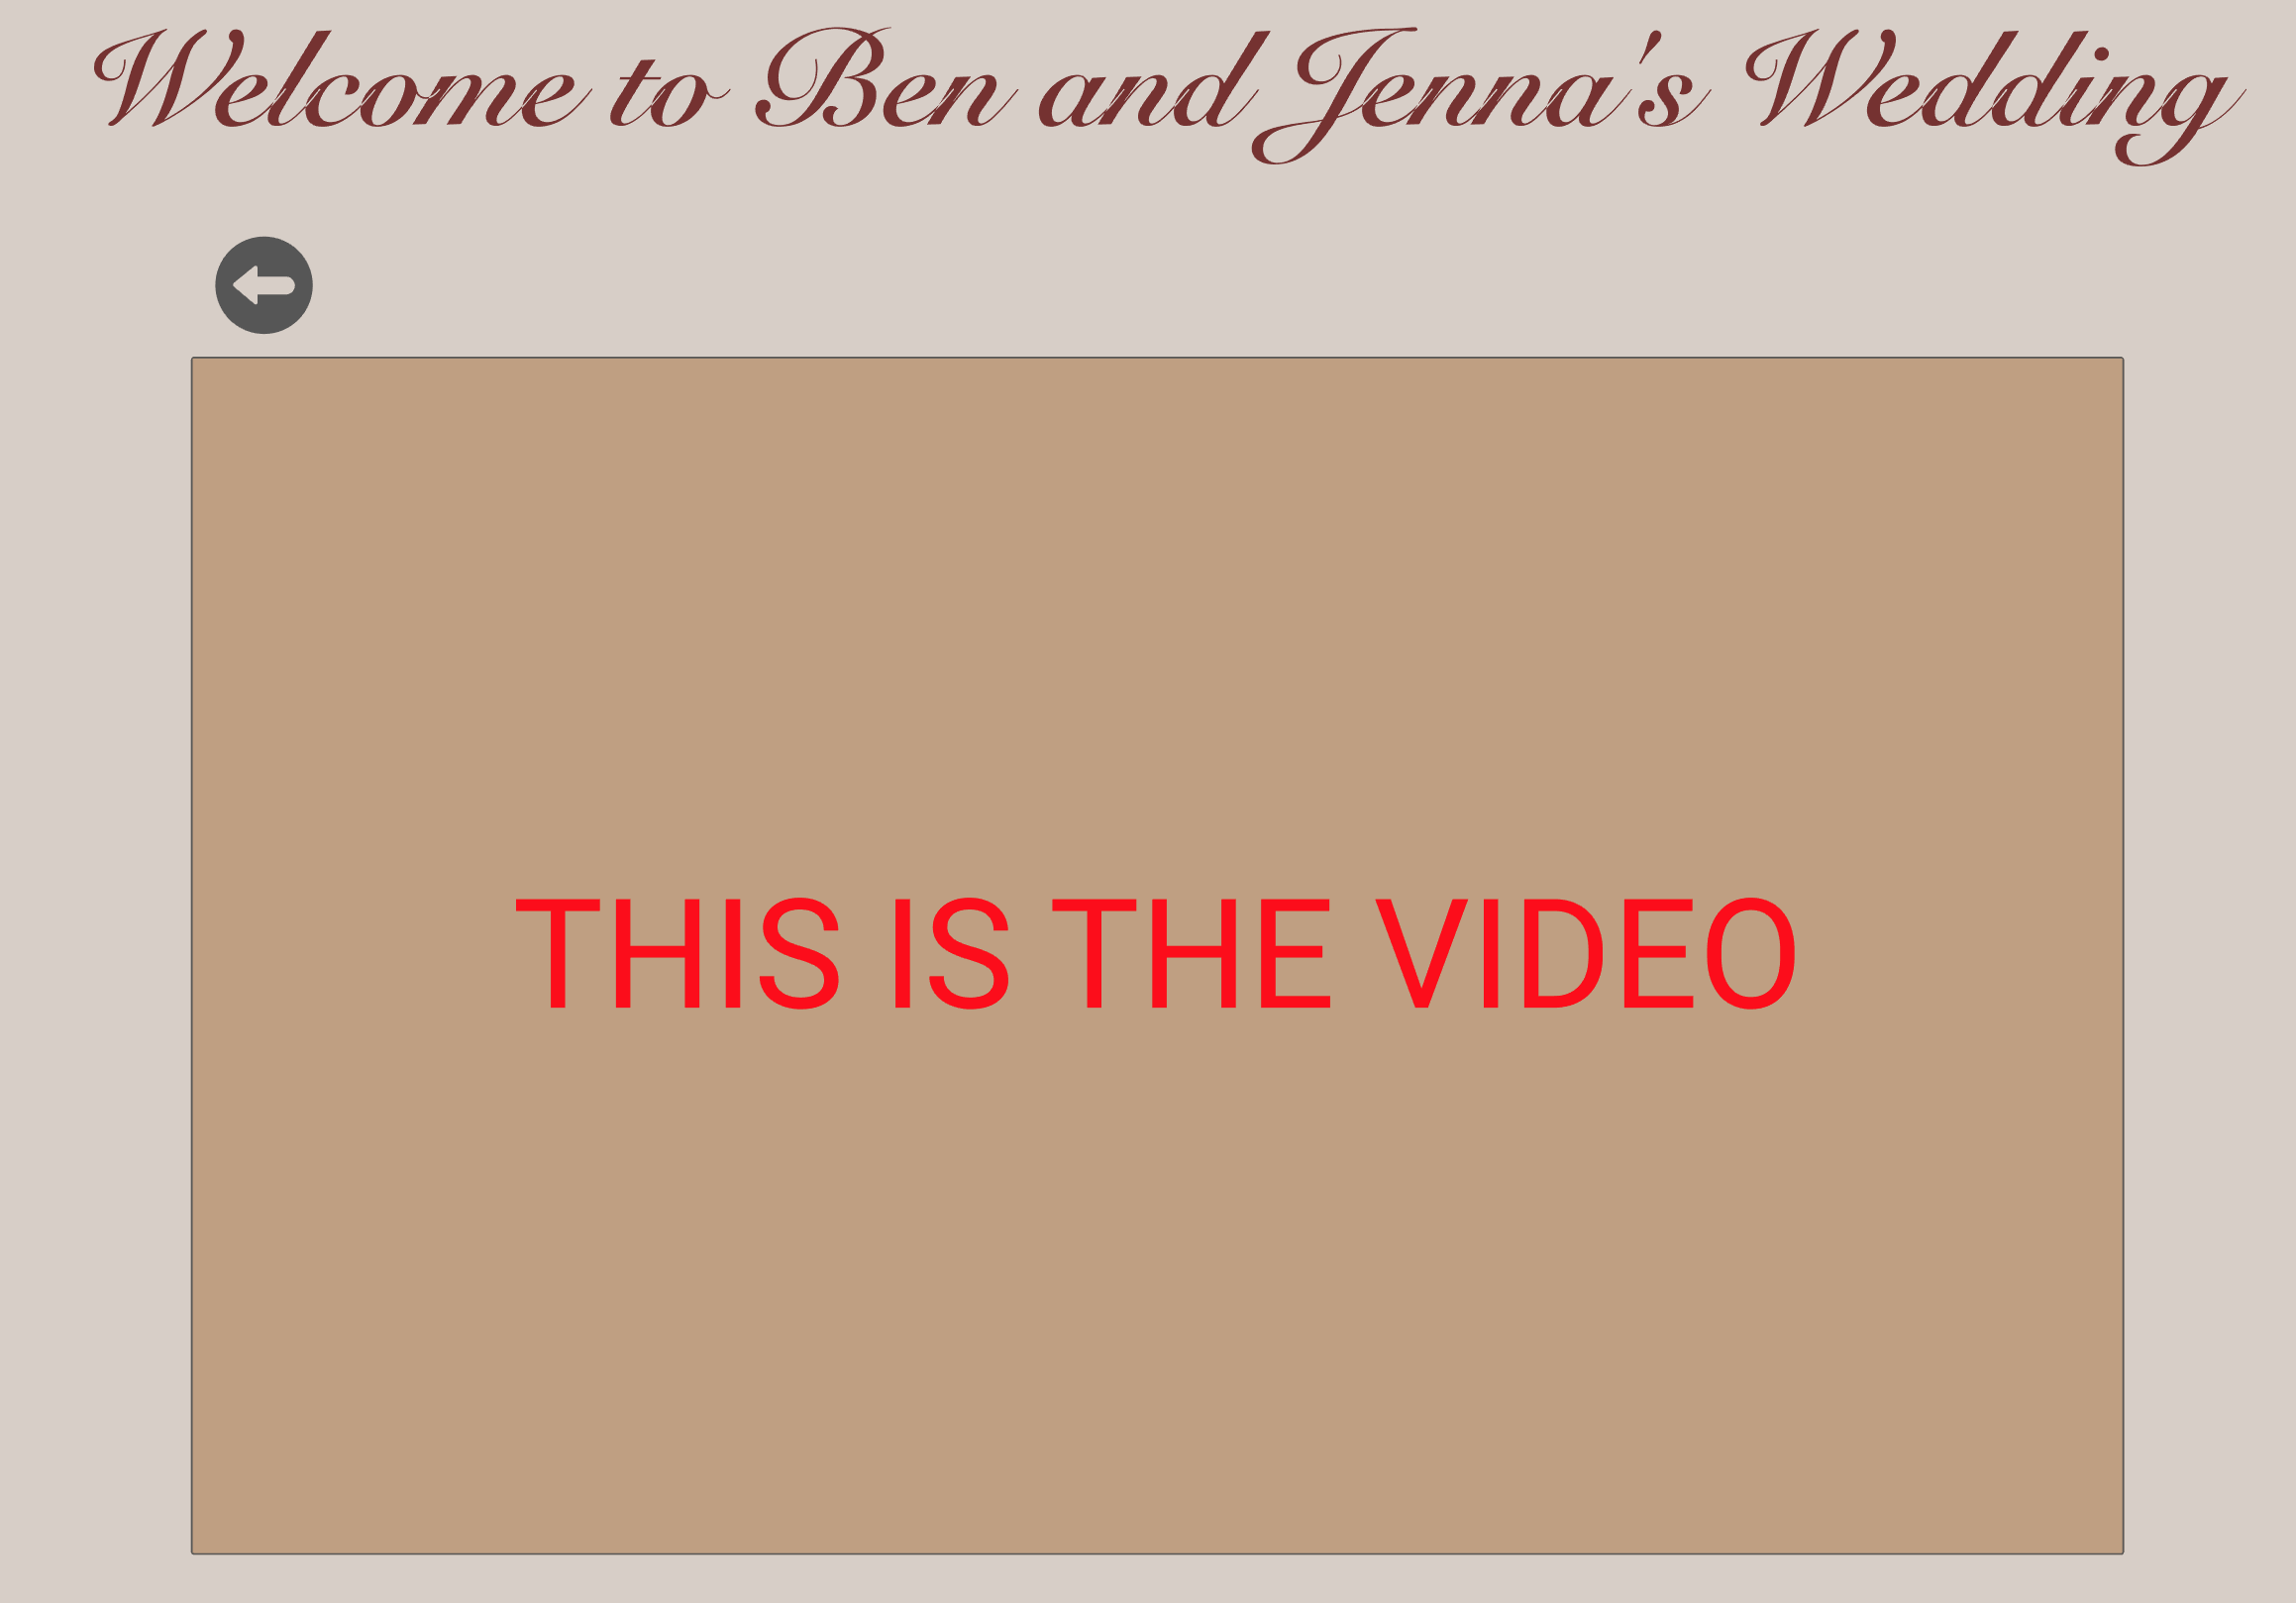
\includegraphics[scale=0.2]{Images/desktop-video.png}
            \centering\caption{Video Page}
            \label{fig:Video}
        \end{figure}
        \begin{figure}[H]
            \centering
            \captionsetup{justification=centering,margin=2cm}
            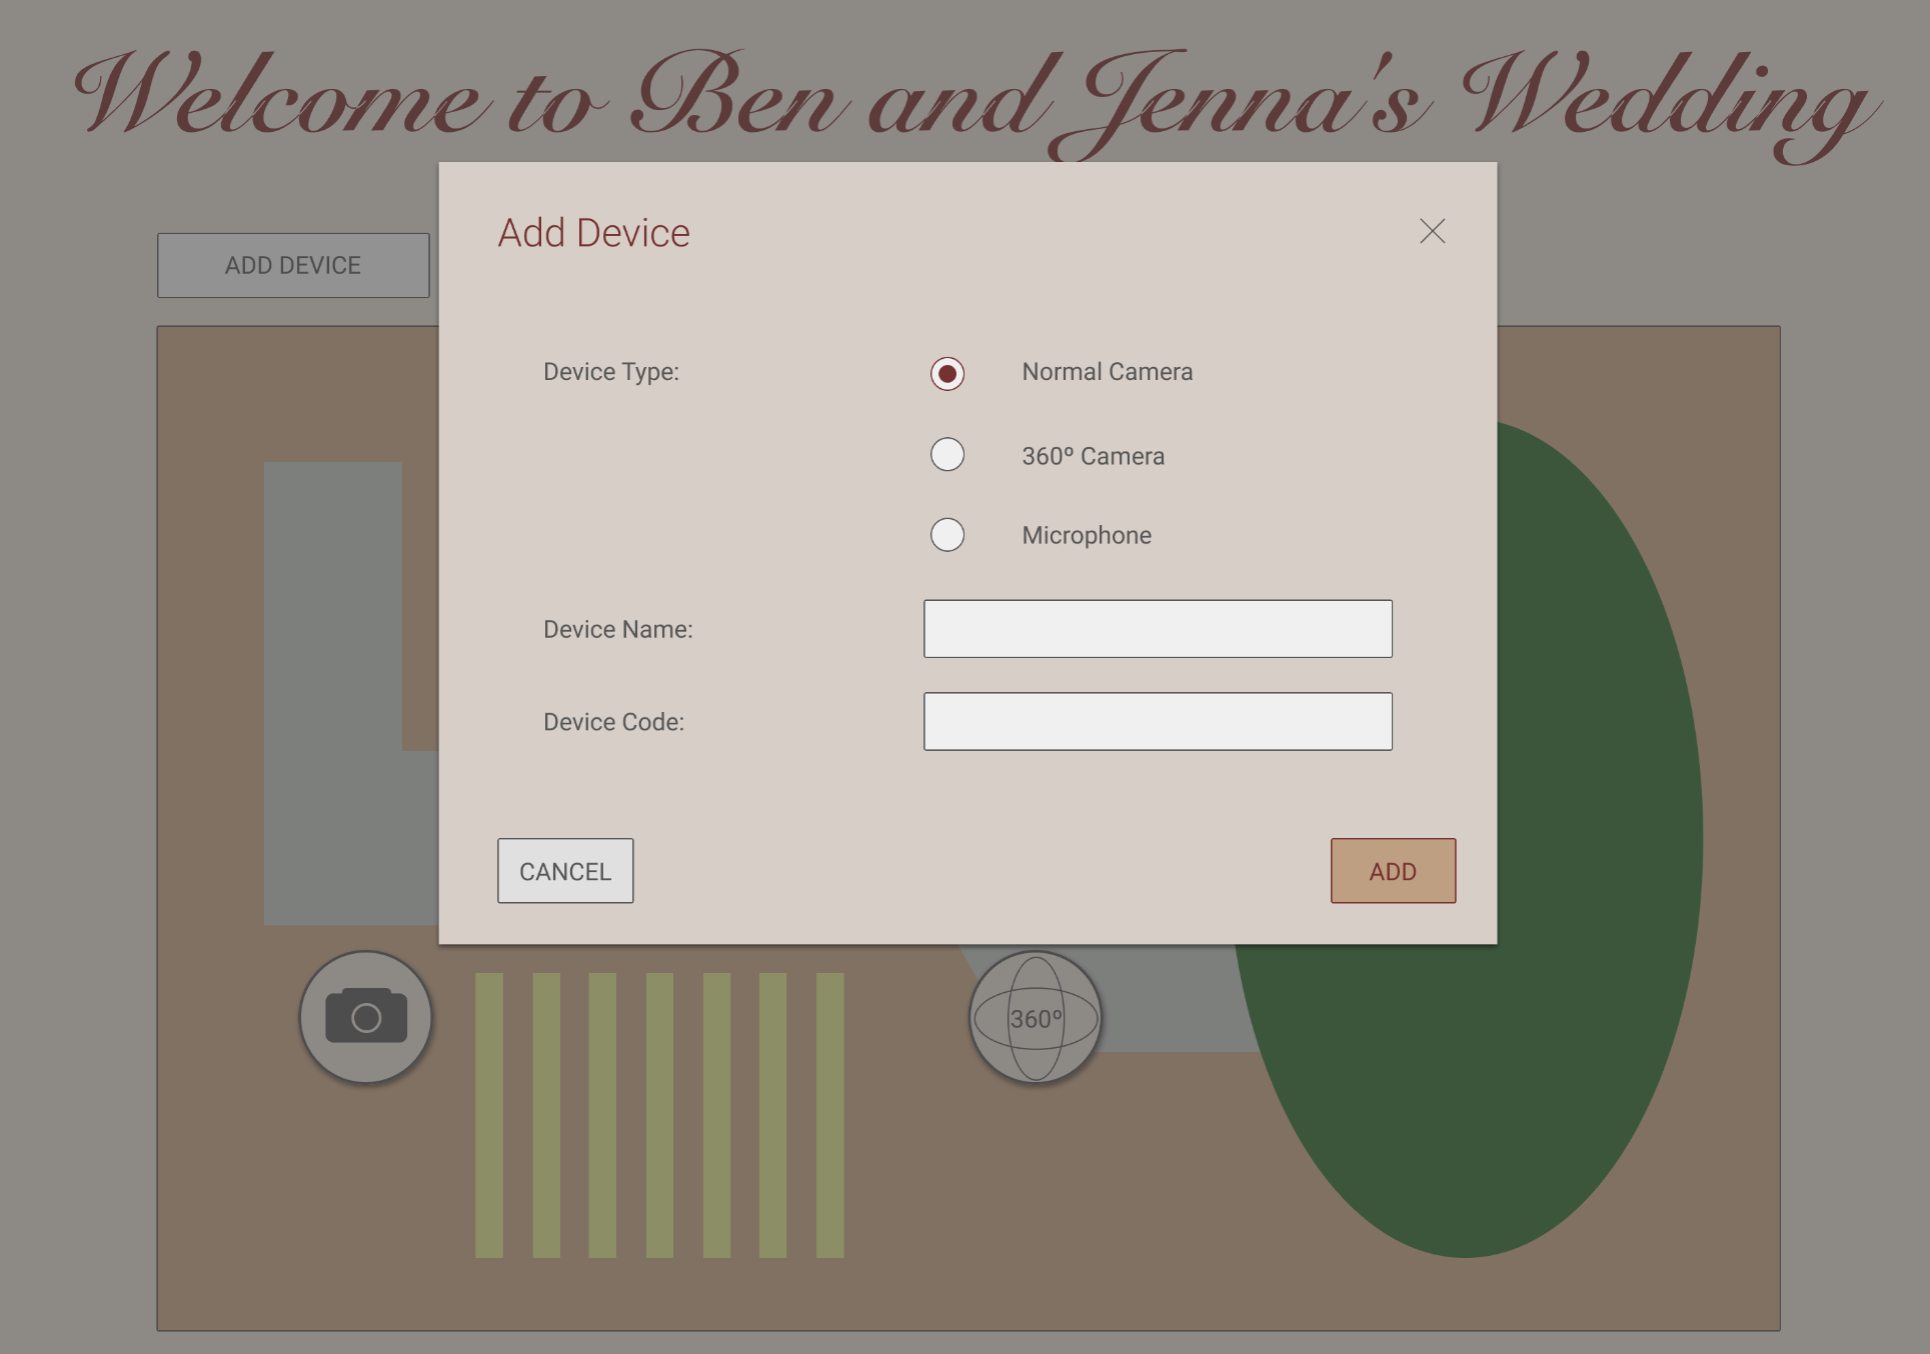
\includegraphics[scale=0.25]{Images/desktop-add.png}
            \centering\caption{Add Modal}
            \label{fig:Add}
        \end{figure}
        \begin{figure}[H]
            \centering
            \captionsetup{justification=centering,margin=2cm}
            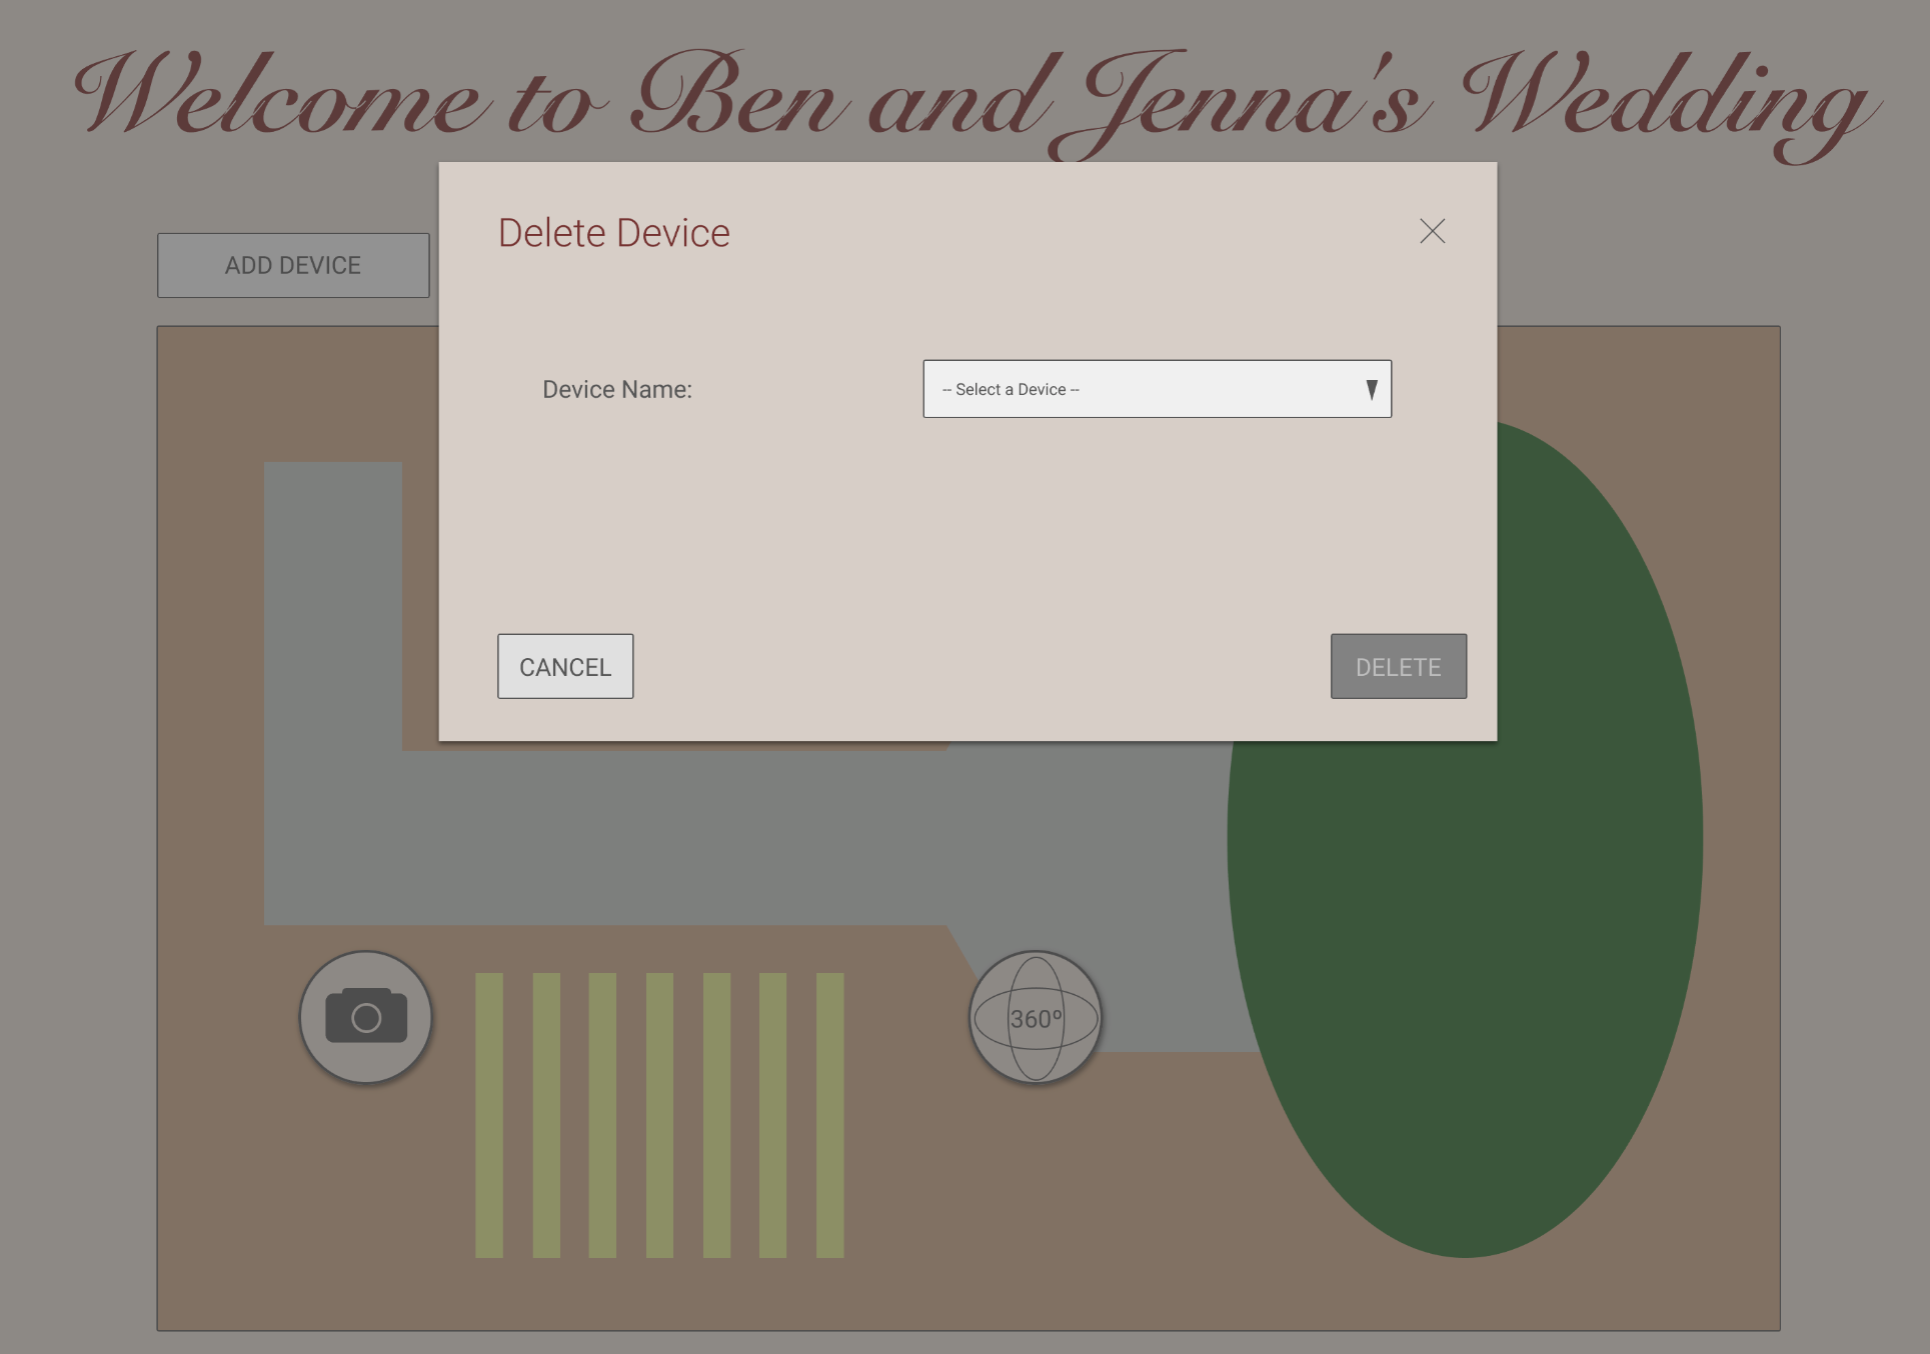
\includegraphics[scale=0.25]{Images/desktop-delete.png}
            \centering\caption{Delete Modal}
            \label{fig:Delete}
        \end{figure}
        \begin{figure}[H]
            \centering
            \captionsetup{justification=centering,margin=2cm}
            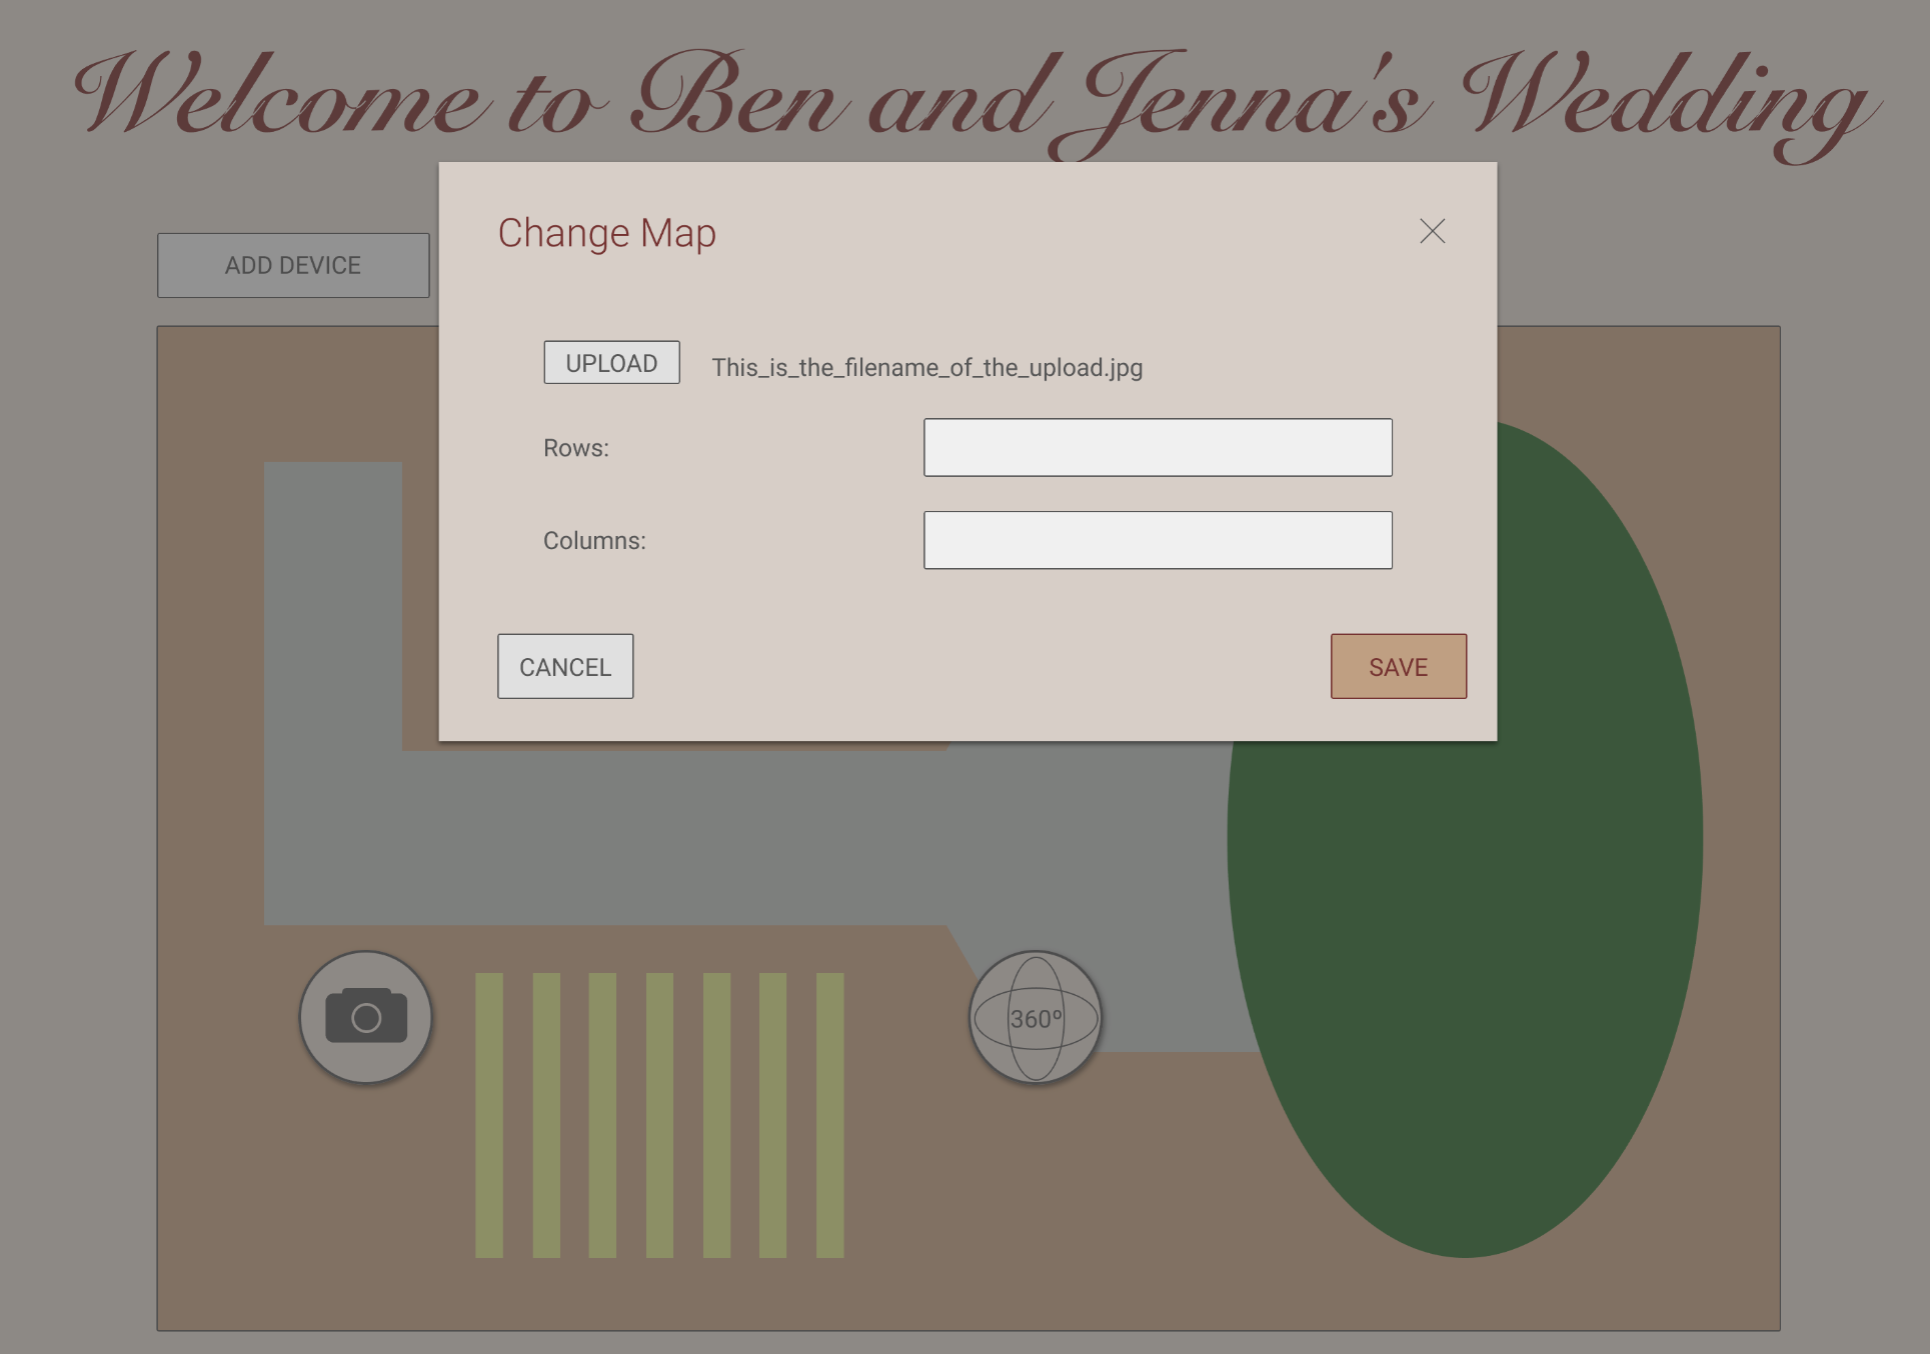
\includegraphics[scale=0.25]{Images/desktop-change.png}
            \centering\caption{Change Map Modal}
            \label{fig:Change}
        \end{figure}
        \begin{figure}[H]
            \centering
            \captionsetup{justification=centering,margin=2cm}
            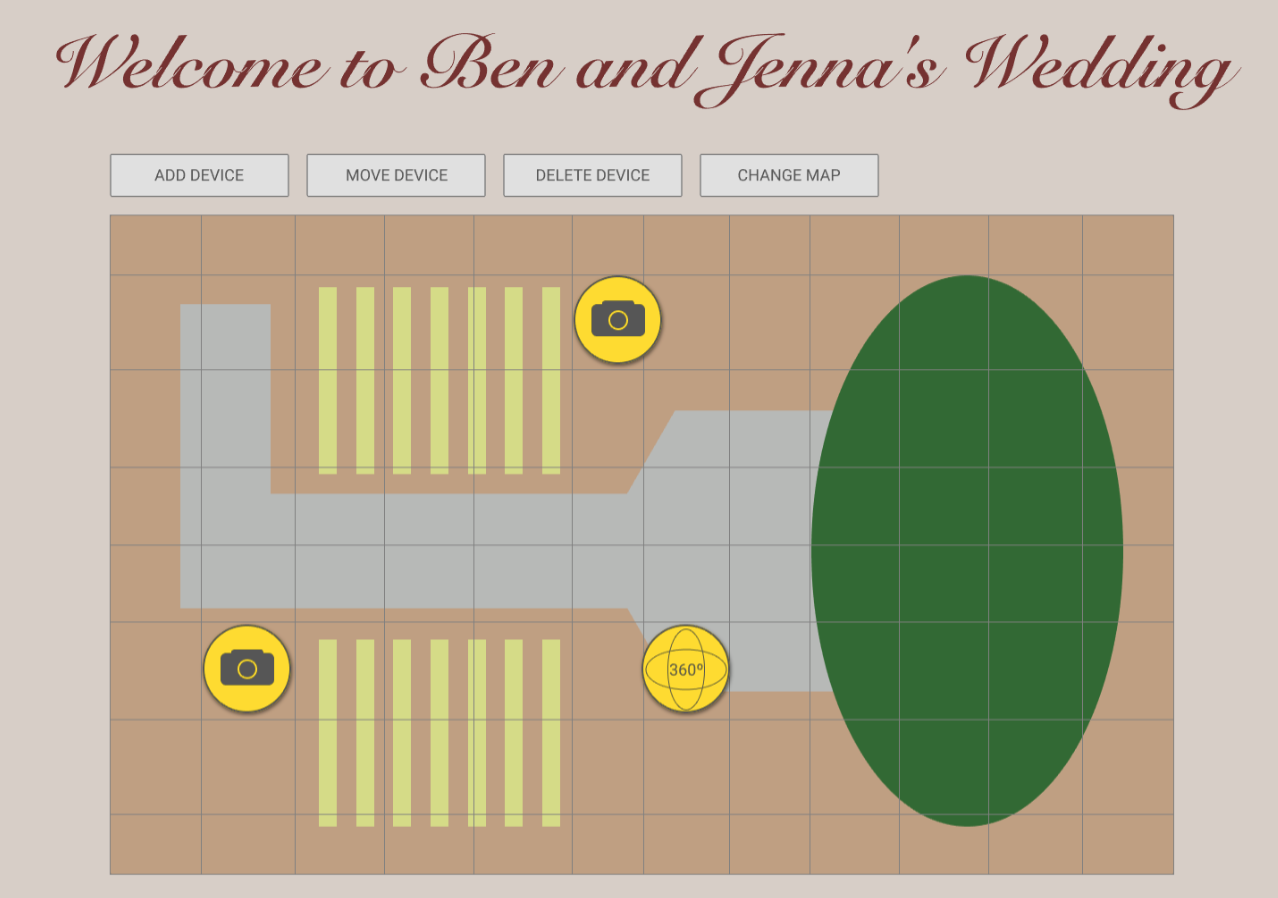
\includegraphics[scale=0.36]{Images/desktop-move.png}
            \centering\caption{Move Device}
            \label{fig:Move}
        \end{figure}
\section{Where we are now}
        Currently, we have a strong foundation for our project.
        We have completed research on the different technologies that we will be using as well as created a time table of when we plan on completing project steps.
        We have a completed prototype and plans to create the actual web portal during winter break. 
        Working on the web page over winter break will give us a good head start for winter term.
\begin{thebibliography}{1}

\bibitem{IEEEhowto:TravelBan}
 Liptak, A. and Shear, M. (2018). Trump’s Travel Ban Is Upheld by Supreme Court. [online] Nytimes.com. Available at: https://www.nytimes.com/2018/06/26/us/politics/supreme-court-trump-travel-ban.html?module=inline [Accessed 12 Oct. 2018].

\end{thebibliography}
\end{document}
